\documentclass[spanish]{article}
\usepackage{titlesec}

%Quitar páginas en blanco
\let\cleardoublepage\clearpage
\usepackage{etoolbox}
\makeatletter
\patchcmd{\@endpart}{\vfil\newpage}{\par}{}{}
\makeatother

%\usepackage[spanish]{babel} ¡Esto estaba interfiriendo con las flechitas de los \tikspicture

\renewcommand{\contentsname}{Índice}

\usepackage[left=4cm, right=4cm]{geometry}
\usepackage{palatino}%Font
\usepackage{graphicx}
\usepackage{wrapfig}
\usepackage{float}
\usepackage{subcaption}
\usepackage{enumitem}
\usepackage{parskip}
\usepackage{multirow}
\usepackage{booktabs}
\usepackage{amsthm}
\usepackage{amssymb}
\usepackage{amsmath}
\usepackage{tikz}
\usepackage{tikz-3dplot}
\usepackage{xcolor}
\usepackage[bookmarks,bookmarksopen,bookmarksdepth=3]{hyperref}
\hypersetup{
	colorlinks=true,
	urlcolor=blue,
	linkcolor=magenta,
	citecolor=blue,
	filecolor=blue,
	urlbordercolor=white,
	linkbordercolor=white,
	citebordercolor=white,
	filebordercolor=white
}

\theoremstyle{definition}
\renewcommand{\proofname}{Demostración}

\newtheorem*{defn}{Definición}
\newtheorem*{lema}{Lema}
\newtheorem*{obs}{Observación}
\newtheorem*{teo}{Teorema}
\newtheorem*{prop}{Proposición}
\newtheorem*{coro}{Corolario}
\newtheorem*{af}{Afirmación}
\newtheorem*{ejer}{Ejercicio}
\newtheorem*{ejem}{Ejemplo}
\newtheorem*{pregunta}{Pregunta}
\newtheorem*{Wreg}{Construcción de Wythoff para poliedros regulares}
\newtheorem*{Wqui}{Construcción de Wythoff para poliedros quirales}

\newcommand{\R}{\mathbb{R}}
\newcommand{\Z}{\mathbb{Z}}
\newcommand{\N}{\mathbb{N}}
\newcommand{\C}{\mathbb{C}}
\newcommand{\Q}{\mathbb{Q}}
\newcommand{\s}{\mathbb{S}}
\newcommand{\PP}{\mathbb{P}}
\newcommand{\p}{\mathcal{P}}
\newcommand{\T}{\mathcal{T}}
\DeclareMathOperator{\img}{img}
\DeclareMathOperator{\Fix}{Fix}
\DeclareMathOperator{\Stab}{Stab}

%\definecolor{blue-violet}{rgb}{0.54, 0.17, 0.89}
\definecolor{azure}{rgb}{0.0, 0.5, 1.0}
\definecolor{green(ncs)}{rgb}{0.0, 0.62, 0.42}
\definecolor{forestgreen(web)}{rgb}{0.13, 0.55, 0.13}
\definecolor{limegreen}{rgb}{0.2, 0.8, 0.2}
\definecolor{palatinateblue}{rgb}{0.15, 0.23, 0.89}
\definecolor{trueblue}{rgb}{0.0, 0.45, 0.81}
\definecolor{goldenyellow}{rgb}{1.0, 0.87, 0.0}

\title{Politopos}
\author{}

\begin{document}
	\maketitle
	\phantomsection
	\addcontentsline{toc}{part}{\contentsname}
	\tableofcontents
	\clearpage

\section{El cubo de Roli}
En 2014, J. Bracho, I. Hubard y D. Pellicer encontraron un 4-politopo quiral en $\R^4$. Es el único ejemplo conocido de un 4-politopo en $\R^4$.

Mostramos una construcción muy sencilla de este cubo. Comenzamos con dos coloraciones de las aristas del 4-cubo:

\tdplotsetmaincoords{70}{10} % Set the viewpoint angles (theta, phi)
\[\begin{tikzpicture}[scale=1.3, tdplot_main_coords, line width=2pt, line cap=round]
	% Define cube coordinates for the inner cube (smaller size)
	\coordinate (A) at (-0.5,-0.5,-0.5);
	\coordinate (B) at (-0.5,0.5,-0.5);
	\coordinate (C) at (0.5,0.5,-0.5);
	\coordinate (D) at (0.5,-0.5,-0.5);
	\coordinate (E) at (-0.5,-0.5,0.5);
	\coordinate (F) at (-0.5,0.5,0.5);
	\coordinate (G) at (0.5,0.5,0.5);
	\coordinate (H) at (0.5,-0.5,0.5);
	
	% Define cube coordinates for the outer cube (larger size)
	\coordinate (A2) at (-1.5,-1.5,-1.5);
	\coordinate (B2) at (-1.5,1.5,-1.5);
	\coordinate (C2) at (1.5,1.5,-1.5);
	\coordinate (D2) at (1.5,-1.5,-1.5);
	\coordinate (E2) at (-1.5,-1.5,1.5);
	\coordinate (F2) at (-1.5,1.5,1.5);
	\coordinate (G2) at (1.5,1.5,1.5);
	\coordinate (H2) at (1.5,-1.5,1.5);
	
	% Draw lines connecting the inner and outer cube vertices
	\draw[limegreen] (B2) -- (F2);%This one must be here
	\draw[blue] (B2) -- (C2);%And this one
	\draw[goldenyellow] (A) -- (A2);
	\draw[goldenyellow] (B) -- (B2);
	\draw[goldenyellow] (C) -- (C2);
	\draw[goldenyellow] (D) -- (D2);
	\draw[goldenyellow] (E) -- (E2);
	\draw[goldenyellow] (F) -- (F2);
	\draw[goldenyellow] (G) -- (G2);
	%\draw[limegreen] (H) -- (H2);
	
	% Draw inner cube edges
	%Y
	\draw[red] (C) -- (D);
	\draw[red] (A) -- (B);
	%\draw[red] (E) -- (F);
	%\draw[red] (G) -- (H);
	%Z
	\draw[limegreen] (A) -- (E);
	\draw[limegreen] (B) -- (F);
	\draw[limegreen] (C) -- (G);
	%\draw[blue-violet] (D) -- (H);
	%X
	\draw[blue] (B) -- (C);
	\draw[blue] (D) -- (A);
	\draw[blue] (F) -- (G);
	\draw[blue] (H) -- (E);
	\draw[limegreen] (D) -- (H);%This here
	\draw[red] (E) -- (F);%This ones here
	\draw[red] (G) -- (H);
	
	% Draw outer cube edges with random colors
	%Y
	\draw[red] (C2) -- (D2);
	\draw[red] (A2) -- (B2);
	\draw[red] (E2) -- (F2);
	\draw[red] (G2) -- (H2);
	%Z
	\draw[limegreen] (A2) -- (E2);
	%\draw[blue-violet] (B2) -- (F2);
	\draw[limegreen] (C2) -- (G2);
	\draw[goldenyellow] (H) -- (H2);%And this one here
	\draw[limegreen] (D2) -- (H2);
	%X
	%\draw[blue] (B2) -- (C2);
	\draw[blue] (D2) -- (A2);
	\draw[blue] (F2) -- (G2);
	\draw[blue] (H2) -- (E2);
\end{tikzpicture}\qquad\qquad\qquad\begin{tikzpicture}[scale=1.3, tdplot_main_coords, line width=2pt, line cap=round]
	% Define cube coordinates for the inner cube (smaller size)
	\coordinate (A) at (-0.5,-0.5,-0.5);
	\coordinate (B) at (-0.5,0.5,-0.5);
	\coordinate (C) at (0.5,0.5,-0.5);
	\coordinate (D) at (0.5,-0.5,-0.5);
	\coordinate (E) at (-0.5,-0.5,0.5);
	\coordinate (F) at (-0.5,0.5,0.5);
	\coordinate (G) at (0.5,0.5,0.5);
	\coordinate (H) at (0.5,-0.5,0.5);
	
	% Define cube coordinates for the outer cube (larger size)
	\coordinate (A2) at (-1.5,-1.5,-1.5);
	\coordinate (B2) at (-1.5,1.5,-1.5);
	\coordinate (C2) at (1.5,1.5,-1.5);
	\coordinate (D2) at (1.5,-1.5,-1.5);
	\coordinate (E2) at (-1.5,-1.5,1.5);
	\coordinate (F2) at (-1.5,1.5,1.5);
	\coordinate (G2) at (1.5,1.5,1.5);
	\coordinate (H2) at (1.5,-1.5,1.5);
	
	% Draw lines connecting the inner and outer cube vertices
	\draw[blue] (B2) -- (F2);%This one must be here
	\draw[limegreen] (B2) -- (C2);%And this one
	\draw[blue] (A) -- (A2);
	\draw[red] (B) -- (B2);
	\draw[goldenyellow] (C) -- (C2);
	\draw[limegreen] (D) -- (D2);
	\draw[goldenyellow] (E) -- (E2);
	\draw[limegreen] (F) -- (F2);
	\draw[blue] (G) -- (G2);
	%\draw[limegreen] (H) -- (H2);
	
	% Draw inner cube edges
	%Y
	\draw[red] (C) -- (D);
	\draw[limegreen] (A) -- (B);
	%\draw[red] (E) -- (F);
	%\draw[red] (G) -- (H);
	%Z
	\draw[red] (A) -- (E);
	\draw[goldenyellow] (B) -- (F);
	\draw[limegreen] (C) -- (G);
	%\draw[blue-violet] (D) -- (H);
	%X
	\draw[blue] (B) -- (C);
	\draw[goldenyellow] (D) -- (A);
	\draw[red] (F) -- (G);
	\draw[limegreen] (H) -- (E);
	\draw[blue] (D) -- (H);%This here
	\draw[blue] (E) -- (F);%This ones here
	\draw[goldenyellow] (G) -- (H);
	
	% Draw outer cube edges with random colors
	%Y
	\draw[blue] (C2) -- (D2);
	\draw[goldenyellow] (A2) -- (B2);
	\draw[red] (E2) -- (F2);
	\draw[limegreen] (G2) -- (H2);
	%Z
	\draw[limegreen] (A2) -- (E2);
	%\draw[blue-violet] (B2) -- (F2);
	\draw[red] (C2) -- (G2);
	\draw[red] (H) -- (H2);%And this one here
	\draw[goldenyellow] (D2) -- (H2);
	%X
	%\draw[blue] (B2) -- (C2);
	\draw[red] (D2) -- (A2);
	\draw[goldenyellow] (F2) -- (G2);
	\draw[blue] (H2) -- (E2);
\end{tikzpicture}\]
En cada vértice de cualquiera de las coloraciones inciden cuatro aristas de colores distintos.

En el 4-cubo normal, las caras son 4-ciclos de aristas de dos colores que van alternando. Definamos en el 4-cubo de la derecha que las caras sean los 8-ciclos de aristas de dos colores que van alternando. Aquí están las caras verde-rojo:
\[\begin{tikzpicture}[scale=1.3, tdplot_main_coords, line width=2pt, line cap=round]
	% Define cube coordinates for the inner cube (smaller size)
	\coordinate (A) at (-0.5,-0.5,-0.5);
	\coordinate (B) at (-0.5,0.5,-0.5);
	\coordinate (C) at (0.5,0.5,-0.5);
	\coordinate (D) at (0.5,-0.5,-0.5);
	\coordinate (E) at (-0.5,-0.5,0.5);
	\coordinate (F) at (-0.5,0.5,0.5);
	\coordinate (G) at (0.5,0.5,0.5);
	\coordinate (H) at (0.5,-0.5,0.5);
	
	% Define cube coordinates for the outer cube (larger size)
	\coordinate (A2) at (-1.5,-1.5,-1.5);
	\coordinate (B2) at (-1.5,1.5,-1.5);
	\coordinate (C2) at (1.5,1.5,-1.5);
	\coordinate (D2) at (1.5,-1.5,-1.5);
	\coordinate (E2) at (-1.5,-1.5,1.5);
	\coordinate (F2) at (-1.5,1.5,1.5);
	\coordinate (G2) at (1.5,1.5,1.5);
	\coordinate (H2) at (1.5,-1.5,1.5);
	
	% Draw lines connecting the inner and outer cube vertices
	\draw[limegreen] (B2) -- (F2);
	
	% Draw inner cube edges
	\draw[red] (C) -- (D);
	\draw[red] (A) -- (B);
	\draw[limegreen] (A) -- (E);
	\draw[limegreen] (B) -- (F);
	\draw[limegreen] (C) -- (G);
	\draw[limegreen] (D) -- (H);
	\draw[red] (E) -- (F);
	\draw[red] (G) -- (H);
	
	% Draw outer cube edges
	\draw[red] (C2) -- (D2);
	\draw[red] (A2) -- (B2);
	\draw[red] (E2) -- (F2);
	\draw[red] (G2) -- (H2);
	\draw[limegreen] (A2) -- (E2);
	\draw[limegreen] (C2) -- (G2);
	\draw[limegreen] (D2) -- (H2);
\end{tikzpicture}\qquad\qquad\qquad\begin{tikzpicture}[scale=1.3, tdplot_main_coords, line width=2pt, line cap=round]
	% Define cube coordinates for the inner cube (smaller size)
	\coordinate (A) at (-0.5,-0.5,-0.5);
	\coordinate (B) at (-0.5,0.5,-0.5);
	\coordinate (C) at (0.5,0.5,-0.5);
	\coordinate (D) at (0.5,-0.5,-0.5);
	\coordinate (E) at (-0.5,-0.5,0.5);
	\coordinate (F) at (-0.5,0.5,0.5);
	\coordinate (G) at (0.5,0.5,0.5);
	\coordinate (H) at (0.5,-0.5,0.5);
	
	% Define cube coordinates for the outer cube (larger size)
	\coordinate (A2) at (-1.5,-1.5,-1.5);
	\coordinate (B2) at (-1.5,1.5,-1.5);
	\coordinate (C2) at (1.5,1.5,-1.5);
	\coordinate (D2) at (1.5,-1.5,-1.5);
	\coordinate (E2) at (-1.5,-1.5,1.5);
	\coordinate (F2) at (-1.5,1.5,1.5);
	\coordinate (G2) at (1.5,1.5,1.5);
	\coordinate (H2) at (1.5,-1.5,1.5);
	
	% Draw lines connecting the inner and outer cube vertices
	\draw[limegreen] (B2) -- (C2);%And this one
	\draw[red] (B) -- (B2);
	\draw[limegreen] (D) -- (D2);
	\draw[limegreen] (F) -- (F2);
	%\draw[limegreen] (H) -- (H2);
	
	% Draw inner cube edges
	%Y
	\draw[red] (C) -- (D);
	\draw[limegreen] (A) -- (B);
	%\draw[red] (E) -- (F);
	%\draw[red] (G) -- (H);
	%Z
	\draw[red] (A) -- (E);
	\draw[limegreen] (C) -- (G);
	%\draw[blue-violet] (D) -- (H);
	%X
	\draw[red] (F) -- (G);
	\draw[limegreen] (H) -- (E);
	
	% Draw outer cube edges with random colors
	%Y
	\draw[red] (E2) -- (F2);
	\draw[limegreen] (G2) -- (H2);
	%Z
	\draw[limegreen] (A2) -- (E2);
	%\draw[blue-violet] (B2) -- (F2);
	\draw[red] (C2) -- (G2);
	\draw[red] (H) -- (H2);%And this one here
	%X
	%\draw[blue] (B2) -- (C2);
	\draw[red] (D2) -- (A2);
\end{tikzpicture}\]

Ahora las facetas: en ambos cubos definamos las facetas como las componentes conexas de tres colores. Aquí están las facetas verde-rojo-azul:
\[\begin{tikzpicture}[scale=1.3, tdplot_main_coords, line width=2pt, line cap=round]
	% Define cube coordinates for the inner cube (smaller size)
	\coordinate (A) at (-0.5,-0.5,-0.5);
	\coordinate (B) at (-0.5,0.5,-0.5);
	\coordinate (C) at (0.5,0.5,-0.5);
	\coordinate (D) at (0.5,-0.5,-0.5);
	\coordinate (E) at (-0.5,-0.5,0.5);
	\coordinate (F) at (-0.5,0.5,0.5);
	\coordinate (G) at (0.5,0.5,0.5);
	\coordinate (H) at (0.5,-0.5,0.5);
	
	% Define cube coordinates for the outer cube (larger size)
	\coordinate (A2) at (-1.5,-1.5,-1.5);
	\coordinate (B2) at (-1.5,1.5,-1.5);
	\coordinate (C2) at (1.5,1.5,-1.5);
	\coordinate (D2) at (1.5,-1.5,-1.5);
	\coordinate (E2) at (-1.5,-1.5,1.5);
	\coordinate (F2) at (-1.5,1.5,1.5);
	\coordinate (G2) at (1.5,1.5,1.5);
	\coordinate (H2) at (1.5,-1.5,1.5);
	
	% Draw lines connecting the inner and outer cube vertices
	\draw[limegreen] (B2) -- (F2);%This one must be here
	\draw[blue] (B2) -- (C2);%And this one
	%\draw[limegreen] (H) -- (H2);
	
	% Draw inner cube edges
	%Y
	\draw[red] (C) -- (D);
	\draw[red] (A) -- (B);
	%\draw[red] (E) -- (F);
	%\draw[red] (G) -- (H);
	%Z
	\draw[limegreen] (A) -- (E);
	\draw[limegreen] (B) -- (F);
	\draw[limegreen] (C) -- (G);
	%\draw[blue-violet] (D) -- (H);
	%X
	\draw[blue] (B) -- (C);
	\draw[blue] (D) -- (A);
	\draw[blue] (F) -- (G);
	\draw[blue] (H) -- (E);
	\draw[limegreen] (D) -- (H);%This here
	\draw[red] (E) -- (F);%This ones here
	\draw[red] (G) -- (H);
	
	% Draw outer cube edges with random colors
	%Y
	\draw[red] (C2) -- (D2);
	\draw[red] (A2) -- (B2);
	\draw[red] (E2) -- (F2);
	\draw[red] (G2) -- (H2);
	%Z
	\draw[limegreen] (A2) -- (E2);
	%\draw[blue-violet] (B2) -- (F2);
	\draw[limegreen] (C2) -- (G2);
	\draw[limegreen] (D2) -- (H2);
	%X
	%\draw[blue] (B2) -- (C2);
	\draw[blue] (D2) -- (A2);
	\draw[blue] (F2) -- (G2);
	\draw[blue] (H2) -- (E2);
\end{tikzpicture}\qquad\qquad\qquad\begin{tikzpicture}[scale=1.3, tdplot_main_coords, line width=2pt, line cap=round]
	% Define cube coordinates for the inner cube (smaller size)
	\coordinate (A) at (-0.5,-0.5,-0.5);
	\coordinate (B) at (-0.5,0.5,-0.5);
	\coordinate (C) at (0.5,0.5,-0.5);
	\coordinate (D) at (0.5,-0.5,-0.5);
	\coordinate (E) at (-0.5,-0.5,0.5);
	\coordinate (F) at (-0.5,0.5,0.5);
	\coordinate (G) at (0.5,0.5,0.5);
	\coordinate (H) at (0.5,-0.5,0.5);
	
	% Define cube coordinates for the outer cube (larger size)
	\coordinate (A2) at (-1.5,-1.5,-1.5);
	\coordinate (B2) at (-1.5,1.5,-1.5);
	\coordinate (C2) at (1.5,1.5,-1.5);
	\coordinate (D2) at (1.5,-1.5,-1.5);
	\coordinate (E2) at (-1.5,-1.5,1.5);
	\coordinate (F2) at (-1.5,1.5,1.5);
	\coordinate (G2) at (1.5,1.5,1.5);
	\coordinate (H2) at (1.5,-1.5,1.5);
	
	% Draw lines connecting the inner and outer cube vertices
	\draw[blue] (B2) -- (F2);%This one must be here
	\draw[limegreen] (B2) -- (C2);%And this one
	\draw[blue] (A) -- (A2);
	\draw[red] (B) -- (B2);
	\draw[limegreen] (D) -- (D2);
	\draw[limegreen] (F) -- (F2);
	\draw[blue] (G) -- (G2);
	%\draw[limegreen] (H) -- (H2);
	
	% Draw inner cube edges
	%Y
	\draw[red] (C) -- (D);
	\draw[limegreen] (A) -- (B);
	%\draw[red] (E) -- (F);
	%\draw[red] (G) -- (H);
	%Z
	\draw[red] (A) -- (E);
	\draw[limegreen] (C) -- (G);
	%\draw[blue-violet] (D) -- (H);
	%X
	\draw[blue] (B) -- (C);
	\draw[red] (F) -- (G);
	\draw[limegreen] (H) -- (E);
	\draw[blue] (D) -- (H);%This here
	\draw[blue] (E) -- (F);%This ones here
	
	
	% Draw outer cube edges with random colors
	%Y
	\draw[blue] (C2) -- (D2);
	\draw[red] (E2) -- (F2);
	\draw[limegreen] (G2) -- (H2);
	%Z
	\draw[limegreen] (A2) -- (E2);
	%\draw[blue-violet] (B2) -- (F2);
	\draw[red] (C2) -- (G2);
	\draw[red] (H) -- (H2);%And this one here
	%X
	%\draw[blue] (B2) -- (C2);
	\draw[red] (D2) -- (A2);
	\draw[blue] (H2) -- (E2);
\end{tikzpicture}\]
El cubo de la derecha se llama Cubo de Roli. Como dijimos, es un 4-politopo quiral. Parece que tiene la mitad de caras y la mitad de facetas de lo que tiene el 4-cubo. Las facetas son poliedros quirales (combintorialmente regulares). Esta construicción se pudo generalizar para crear otros poliedros quirales, como mostramos en la siguiente sección.

\section{Resumen: Quiral polyhedra from a PC construction}
Dado un 4-politopo regular $\mathcal{T}$, la construcción central es:
\begin{enumerate}
	\item Calcular el poliedro de Petrie-Coxeter $PC_\alpha(\mathcal{T})$. Resulta ser regular o de clase $2_{\{0,2\}}$.
	\item Aplicar la halving operation para obtener $PC_\alpha(\mathcal{T})^\eta$.
	\item Aplicar la operación de 2-facetting (2-hole) para obtener $(PC_\alpha(\mathcal{T})^\eta)^\phi:=H_\alpha(\mathcal{T})$. Éste es un poliedro regular o quiral.
\end{enumerate}
Cuando comenzamos con el 4-cubo, para \textcolor{azure}{ciertos valores de $\alpha$ (creo que 1 o 2)} obtenemos las facetas del Cubo de Roli.

A continuación desglosaremos este proceso.

\subsection{Definiciones}

\begin{defn}Un poliedro $\p$ es
\begin{itemize}
	\item \textbf{regular} (resp. \textbf{combinatoriamente regular}) si su grupo de simetrías $G(\p)$ (resp. grupo de automorfismos $\Gamma(\p))$ actúa transitivamente en las banderas .
	\item \textbf{quiral} (resp. \textbf{combinatoriamente quiral}) si $G(\p)$ (resp. $\Gamma(\p)$) induce dos órbitas en las banderas con la propiedad de que dos banderas adyacentes están en órbitas diferentes.
\end{itemize}
\end{defn}
\begin{obs}
	Si $\p$ es regular o quiral, el grupo de simetrías actúa transitivamente en caras, aristas y vértices.
\end{obs}

\subsection{La construcción de Petrie-Coxeter}
\begin{figure}[H]
	\centering
	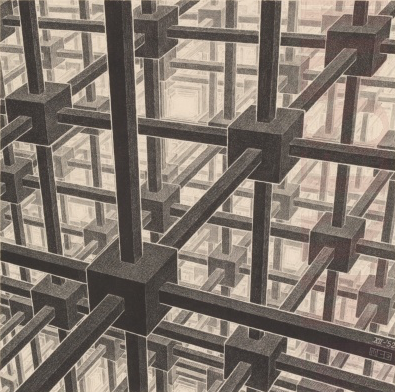
\includegraphics[width=0.45\linewidth]{p2}
	\caption*{La construcción de Petrie-Coxeter y los valores de $\alpha$.}
\end{figure}
Dado un 4-politopo regular $\T$, mostraremos cómo constuir un poliedro regular o quiral $PC(\T)$. Suponemos por el resto del texto que $\T$ tiene caras planas.

Se escoge número $\alpha$ entre 0 y 1. Para un vértice $v$ de $\T$ y una cara que contiene a $v$, definimos el punto $(v,c)_\alpha$ sobre el segmento que une $v$ con $c$ a distancia $d\alpha$ desde $v$, donde $d$ es la distancia entre ellos. Estos puntos serán los vértices del poliedro $PC_\alpha(\T)$.

Las aristas son (1) los segmentos que unen $(v,c)_\alpha$ con $(v',c)_\alpha$, donde $v$ y $v'$ son vértices en una misma arista de $\T$; y (2) los semgentos que unen  $(v,c)_\alpha$ con $(v,c')_\alpha$ donde $c$ y $c'$ son facetas que comparten una cara conde está $v$.

Las caras son los cuadrados $(v,c)_\alpha$, $(v',c)_\alpha$, $(v,c')_\alpha$ y $(v',c')_\alpha$ donde $c$ y $c'$ son caras que contienen a la arista entre $v$ y $v'$.

\begin{figure}[H]
	\centering
	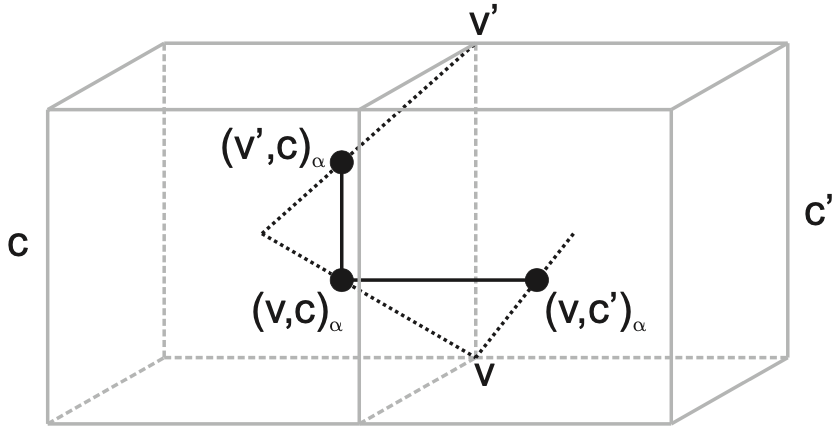
\includegraphics[width=0.5\linewidth]{p3}
\end{figure}
Tenemos algunos resultados sobre esta construcción:
\begin{teo}
	Para cualquier $\alpha\in(0,1)$ y cualquier politopo regular $\T$, $PC_\alpha(\T)$ es un poliedro.
\end{teo}
\begin{obs}
	Para cualesquiera $\alpha\in(0,1)$, un 4-politopo regular $\T$ y su dual $\T^*$, $PC_\alpha(\T)=PC_{1-\alpha}(\T)$.
\end{obs}
\begin{teo}
	Para cualesquiera $\alpha\in(0,1)$, un 4-politopo regular $\T$, el grupo de simetría de $\T$ es isomorfo a un subgrupo de índice a lo más 2 de $G(PC_\alpha(\T))$. Además, $PC_\alpha(\T)$ es regular o un poliedro de dos órbitas en la clase $2_{\{0,2\}}$.
\end{teo}

\subsection{Halving operation}
\tdplotsetmaincoords{70}{15} % Set the viewpoint angles (theta, phi)
\[\begin{tikzpicture}[scale=3, tdplot_main_coords, line width=2pt, line cap=round]
	% Define cube coordinates for the inner cube (smaller size)
	\coordinate (A) at (-0.5,-0.5,-0.5);
	\coordinate (B) at (-0.5,0.5,-0.5);
	\coordinate (C) at (0.5,0.5,-0.5);
	\coordinate (D) at (0.5,-0.5,-0.5);
	\coordinate (E) at (-0.5,-0.5,0.5);
	\coordinate (F) at (-0.5,0.5,0.5);
	\coordinate (G) at (0.5,0.5,0.5);
	\coordinate (H) at (0.5,-0.5,0.5);
	
	% Draw inner cube edges
	\draw[limegreen] (C) -- (D);
	\draw[limegreen] (A) -- (B);
	\draw[limegreen] (A) -- (E);
	\draw[limegreen] (B) -- (F);
	\draw[limegreen] (C) -- (G);
	\draw[limegreen] (B) -- (C);
	\draw[limegreen] (D) -- (A);
	\draw[limegreen] (F) -- (G);
	\draw[limegreen] (H) -- (E);
	\draw[limegreen] (D) -- (H);
	\draw[limegreen] (E) -- (F);
	\draw[limegreen] (G) -- (H);
	
	\draw[blue] (A) -- (H);
	\draw[blue] (F) -- (H);
	\draw[blue] (F) -- (A);
	\draw[blue] (C) -- (H);
	\draw[blue] (A) -- (C);
	\draw[blue] (F) -- (C);
\end{tikzpicture}\]
Esta operación transforma un poliedro $\p$ con caras cuadradas en otro poliedro $\p^\eta$, cuyos vértices son algunos de los vértices de $\p$, donde dos de ellos son adyacentes si y sólo si son vértices opuestos en una cara de $\p$. Las caras de $\p^\eta$ con figuras de vértice de algunos de los vértices de $\p$.

Como $PC_\alpha(\T)$ tiene caras cuadradas, le podemos aplicar esta operación. Y como además es regular o de clase $2_{\{0,2\}}$, cualquier de los resultados de aplicarle la operación Halving son isomorfos.


\subsection{2-Hole}
A 2-hole is constructed by traversing an edge to one of its endpoints, skipping the first edge on the left according to some local orientation, and then traversing a second edge. This procedure is repeated until an edge is traversed twice in the same direction.

La operación Facetting o 2-Hole convierte un poliedro $\p$ con vértices de grado al menos 5 en una estructura $\p^\phi$ cuyo 1-esqueleto está contenido en el 1-esqueleto de $\p$ y sus caras son un subconjunto de los 2-hoyos de $\p$.

Dados un vértice, arista y 2-hoyo incidentes, se va construyendo $\p^\phi$ por pasos de forma que el 1-esqueleto sea conexo y cada arista pertenezca a exactamente dos 2-hoyos. El resultado no siempre es un poliedro, pero en nuestro caso sí lo es. Esto es consecuencia del siguiente resultado:

\begin{teo}
	Cuando $PC_\alpha(\T)^\eta$ es un poliedro, es regular o de clase $2_{\{1\}}$.
\end{teo}

\begin{figure}[H]
	\centering
	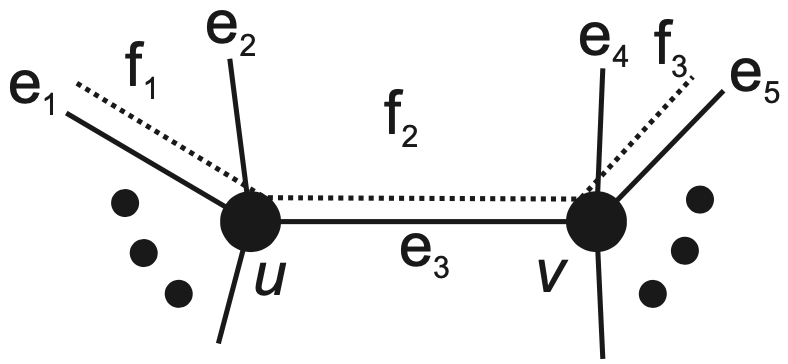
\includegraphics[width=0.5\linewidth]{p4}
	\caption*{Construcción de un 2-hoyo}
\end{figure}

\subsection{Los quiralitos}
Finalmente podemos definir
\[H_\alpha(\T)=\left(PC_\alpha(\T)^\eta\right)^\phi\]
Para entender cómo construir los grupos de simetrías de los quiralitos, debemos recordar algunas cosas. Dado un poliedro $\p$ regular o quiral, el subgrupo de automorfismos $\Gamma^+(\p)$ está generado por dos rotaciones distinguidas: la de la cara, $\sigma_1$ y la del vértice $\sigma_2$.

Cuando $\p$ es plano (todas sus caras están en un plano, por ejemplo, el hemicubo en $\PP^2$), es posible que haya más de una isometría que actúa como $\sigma_1$ y $\sigma_2$.  Sin embargo, si $\p$ no es plano, son únicas.:
\begin{teo}
	Si $\p$ es un poliedro regular o quiral con caras planas, existen únicas isometrías $S_1$ y $S_2$ que actúan como $\sigma_1$ y $\sigma_2$ con respecto a alguna bandera base $\Phi$.
\end{teo}
Y luego,
\begin{prop}
	Si $H_\alpha(\T)$ es un poliedro, es regular o quiral.
\end{prop}
\begin{proof}
	Basta mostrar que existe la rotación de la cara $S_1$ y la rotación del vértice $S_2$. ¿Por qué? Si el grupo de simetrías del poliedro está generado por estas dos simetrías, tenemos que deducir que hay una o dos órbitas en banderas.
\end{proof}

Se hizo este procedimiento para cada uno de los 4-politopos regulares (6 convexos y 10 estrellados). Veamos cómo analizar los poliedros resultantes.

De la regularidad de $\mathcal{T}$ podemos estudiar la simetría de $H_\alpha(\mathcal{T})$. Mientras que $G(\mathcal{T})=\langle R_0,R_1,R_2,R_3\rangle$ como en la construcción Wythoff, resulta que $G(H_\alpha(\mathcal{T}))\leq \langle S_1,S_2\rangle$, donde
\begin{align*}
	S_1&=R_0R_1R_3R_2\\
	S_2&=R_2R_1
\end{align*}
Aquí, $S_1$ es un tornillo y $S_2$ una rotación, dando lugar a la notación $\left\{\frac{p}{p_1,p_2},q\right\}$ donde $q$ es el orden de la rotación y los enteros $p,p_1$ y $p_2$ caracterizan al tornillo. Esto sugiere qué clase de poliedro es $H_\alpha(\mathcal{T})$: tiene caras helicoidales, $q$ en cada vértice.

Se encontraron los siguientes Quiralitos o Halving-2-Holes:

\begin{center}
	\begin{tabular}{|c|c|c|c|c|c|}
		\hline
		&\multirow{2}{*}{4-politopo} &\multirow{2}{*}{Quiralito}&  \multirow{3}{*}{$\#(G)$} &\multirow{3}{*}{$[G:\Gamma^+]$}& Colapsa\\
		&\multirow{2}{*}{ $\T$}&\multirow{2}{*}{$H_\alpha(T)$}&&&cuando\\
		&&&&&$\alpha=(0,1)$ \\
		\hline\hline
		\multirow{5}{*}{\rotatebox{90}{Convexos}}&\{3,3,3\} & $\{\frac{5}{1,2},3\}$ &60& 1 & (4,4) \\
		&\{4,3,3\} & $\{\frac{8}{1,3},3\}$ &48& 4&(1,2) \\
		&\{3,4,3\} & $\{\frac{12}{1,5},4\}$ &192&3&(2,2) \\
		&\{5,3,3\} & $\{\frac{30}{1,11},3\}$ &1440&5&(1,4)\\
		\hline
		\multirow{6}{*}{\rotatebox{90}{Estrellados}}&\{3,5,5/2\} &$\{\frac{20}{1,9},5\}$&1200&6&(2,2)\\
		&\{5,5/2,5\} & $\{\frac{15}{1,4},5/2\}$ &7200&1&(12,12)\\\cline{2-6}
		&\textcolor{magenta}{\{5,3,5/2\}} & $\{\frac{12}{1,5},3\}$ &144&50&(1,1)\\\cline{2-6}
		&\textcolor{magenta}{\{3,3,5/2\}}&$\{\frac{30}{7,13},3\}$& 1440 & 5 &(4,1)\\\cline{2-6}
		&\{3,5/2,5\}& $\{\frac{20}{3,7},5/2\}$ &1200&6& (2,2) \\
		&\{5/2,5,5/2\} & $\{\frac{15}{2,7},5\}$ &7200&1& (12,12)\\
		\hline
	\end{tabular}
\end{center}
Donde $G$ es el grupo de simetrías del quiralito.

Distintos valores de $\alpha$ en la construcción de Petrie-Coxeter dan lugar a distintos poliedros. Hay ciertos valores para los cuales las simetrías que generan $H_\alpha(\mathcal{T})$ son simetrías de $\mathcal{T}$. Cuando $\alpha=0$, los vértices de $PC_\alpha(\mathcal{P})$ son los vértices de $\mathcal{P}$.

Cuando $\alpha=0,1$, es posible que algunos de los vértices en la construcción "colapsen". Eso quiere decir que algunos vértices terminan siendo el mismo, y el resultado puede no ser un poliedro. Si, en cambio, aparece el valor 1, leemos que "la cantidad de vértices que colapsan es 1" (para $\alpha=0$ si el 1 está a la izquierda, y respectivamente $\alpha=1$ derecha). Es decir, no hay colapso.

Conviene entonces estudiar los casos donde no hay colapso para $\alpha=0$ pues en este caso la construcción de Petrie-Coxeter nos devuelve una estructura cuyos vértices son los mismos vértices del 4-politopo. Así, podremos usar las simetrías del 4-politopo original.




%
%En este punto toda la información sobre $H_\alpha(\mathcal{T})$ debe estar al alcance de unas cuentas. Podemos darle coordenadas y encontrar una expresión en forma de orden parcial.
%
%\begin{teo}
%	Cualquier poliedro quiral con caras helicoidales es combinatoriamente regular.
%\end{teo}

\section{Quiralitos estrellados}
Aquí comienza nuestro trabajo, basado en la siguiente sospecha: así como el cubo de Roli es la faceta de un 4-politopo quiral, 

\begin{quote}\textbf{hay tres de los quiralitos que son las facetas de ciertos 4-politopos quirales.}\end{quote}

Los sospechosos son $H_1\{5,3,5/2\}$, $H_0\{5,3,5/2\}$ y $H_1\{3,3,5/2\}$. Se trata de los quiralitos obtenidos a partir de los 4-politopos estrellados "Gran 120-celda" y "Gran 600-celda", resp. Dos de ellos están escogidos para valores de $\alpha=1$, de forma que en estos dos casos estaremos trabajando con los 4-politopos duales, el \{5/2,5,3\} "Pequeño 120-celda estelado" y el \{5/2,3,3\}, "Gran gran 120-celda estelada".

El primer paso es obtener los grupos de estos dos 4-politopos.

\subsection{Del convexo al estrellado}
Comenzamos con el grupo del \{5,3,5/2\}, la gran 120-celda. El grupo se denota [5,3,5/2]. La idea es tomar el grupo de simetrías de alguno de los convexos y expresar las relaciones del estrellado en términos de aquéllas.

En nuestro caso, partimos de que el grupo de la 120-celda, [5,3,3], está generado por $R_0,R_1,R_2$ y $R_3$ como Wythoff, queremos expresar el grupo en términos de cuatro generadores $T_0,T_1,T_2$ y $T_4$. 

Comenzemos en dimensión 3, intentando expresar el [5/3,3] a partir del grupo del dodecaedro. Después de muchos intentos logramos esto:

\begin{center}
	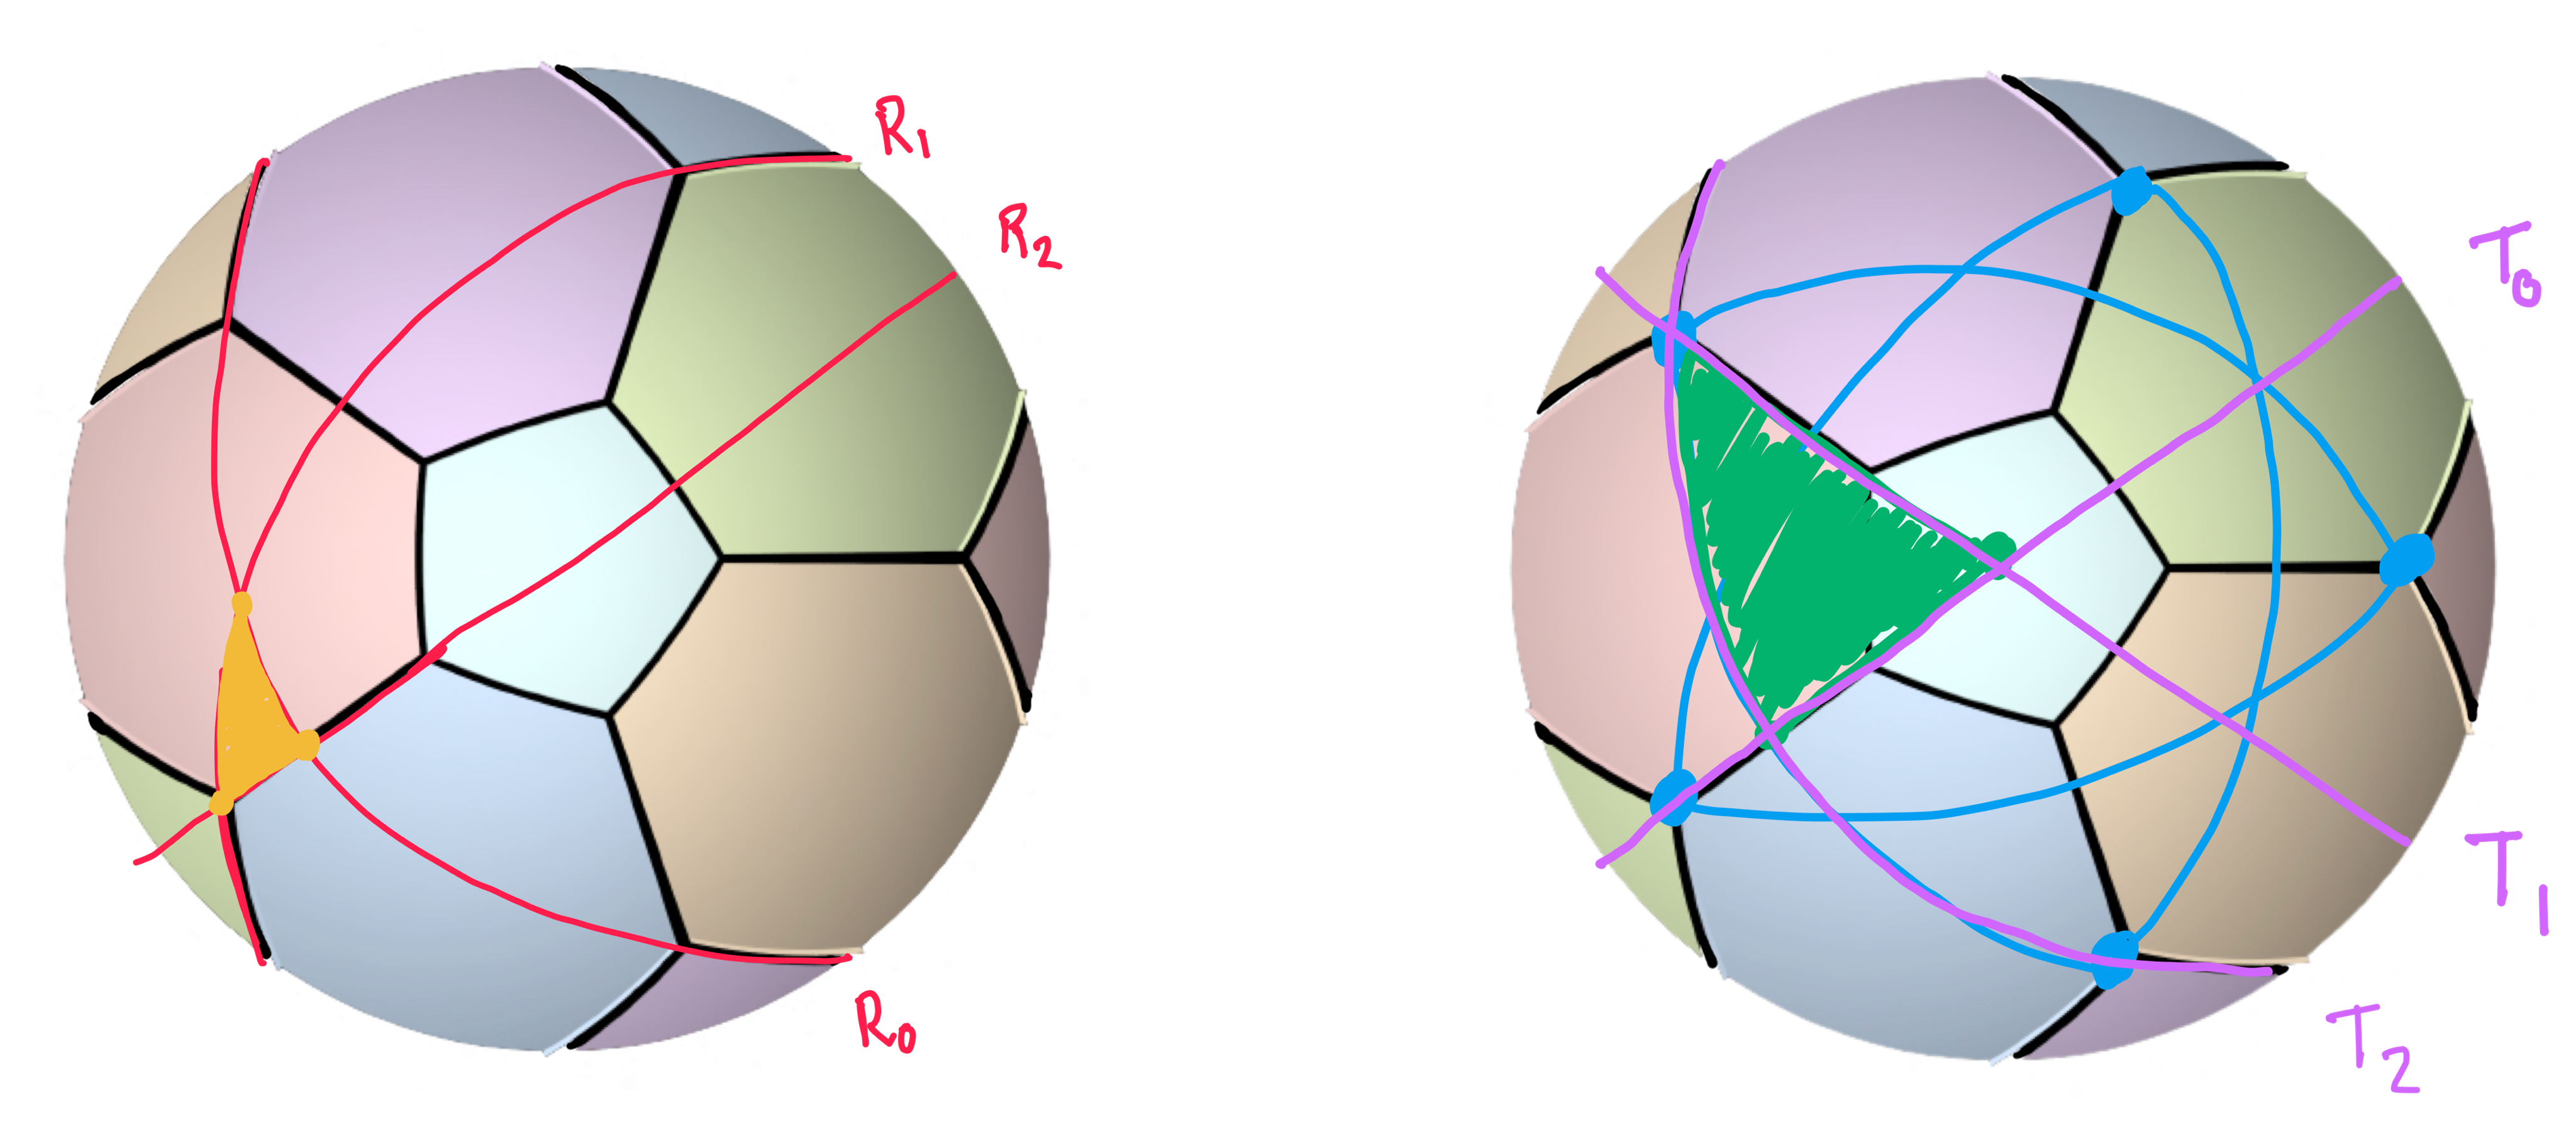
\includegraphics[width=0.9\linewidth]{p1}
\end{center}
Es decir:
\[T_0=R_2,\qquad T_2=R_0,\qquad T_1=(R_0R_1)^2R_2(R_0R_1)^{-2}\]
ya que $T_1$ es rotar $R_2$ en sentido antihorario con centro en el centro de la cara base

Ahora para encontrar la reflexión $T_3$ recordemos que la composición $T_2T_3$ es la rotación en la arista de orden 3. Aunque esta intuición es correcta, \textbf{no es claro cómo encontrar $T_3$ en términos de las $R_i$ con esta información.} ¿Y luego qué pasó?

En los notebooks, resulta que el grupo $[5/2,3,3]=[3,3,5/2]:=\langle T_i\rangle$ está dado en términos del grupo $[5,3,5/2]:=\langle P_i\rangle$ de acuerdo a:
\[T_0=P_3,\qquad T_1=(P_2P_1P_0)P_1(P_2P_1P_0)^{-1},\qquad T_2=P_0,\qquad T_3=(P_1P_0)P_1(P_1P_0)^{-1}\]
¿Qué podemos hacer? Decir cómo están dadas las $P_i$ en términos de las $R_i$ y habríamos terminado. Bueno, de hecho,
\[P_0=R_0,\qquad P_1=(R_1R_2)R_3(R_1R_2)^{-1},\qquad P_2=R_3R_2R_3,\qquad P_3=R_2\]
Así que a la mera hora:
\begin{align*}
	T_0=R_2,\qquad &T_2=R_0,\\
	T_1=\left((R_3R_2R_3)((R_1R_2)R_3(R_1R_2)^{-1})\right)(R_0)&(R_1R_2)R_3(R_1R_2)^{-1}\left(R_3R_2R_3)((R_1R_2)R_3(R_1R_2)^{-1})\right)^{-1},\\
	T_3=\left((R_1R_2)R_3(R_1R_2)^{-1})(R_0)\right)&((R_1R_2)R_3(R_1R_2)^{-1})\left((R_1R_2)R_3(R_1R_2)^{-1})(R_0)\right)^{-1}
\end{align*}
Antes de pasar a estudiar las $T_i$, hicimos esta cuenta con las $P_i$. Tenemos las presentaciones de los grupos:
\label{rels}\begin{align*}
	[3,3,5]=\langle R_i|R_i^2=(R_0R_1)^3=(R_1R_2)^3=(R_2R_3)^5=1\\
	(R_0R_2)^2=(R_0R_3)^2=(R_1R_3)^2=1\rangle\\ \\
	[5,3,5/2]=\langle P_i|P_i^2=(P_0P_1)^5=(P_1P_2)^3=(P_2P_3)^5=1\\
	(P_0P_2)^2=(P_0P_3)^2=(P_1P_3)^2=1\rangle
\end{align*}
Así que hay que checar que las $P_i$ satisfagan eso. \textbf{Se comprobaron todas excepto que $(P_1P_2)^3=1$.}

\paragraph{La búsqueda por la bandera} Se logró identificar cómo está situada la bandera del \{5,3,5/2\} con respecto a la bandera del \{3,3,5\}.

\begin{af}[La idea de Roli] Pensemos que el icosaedrito de los no-vértices del \{5/2,3\} es la figura de vértice del \{3,3,5\}. Al hacer actuar las isometrías $R_i$ sobre el \{5/2,3\} obtenemos el \{5/2,3,5\}
\end{af}
\begin{proof}
	Definamos 
		\[P_0=R_0,\qquad P_2=R_3,\qquad P_3=R_2\]
	Para $P_1$ hay que hacer un poquito más de chamba. Apliquemos primero la rotación en la arista base "hacia nosotros", $R_3R_2$, dos veces:
	\begin{figure}[H]
	\begin{subfigure}{0.4\linewidth}
		\centering
		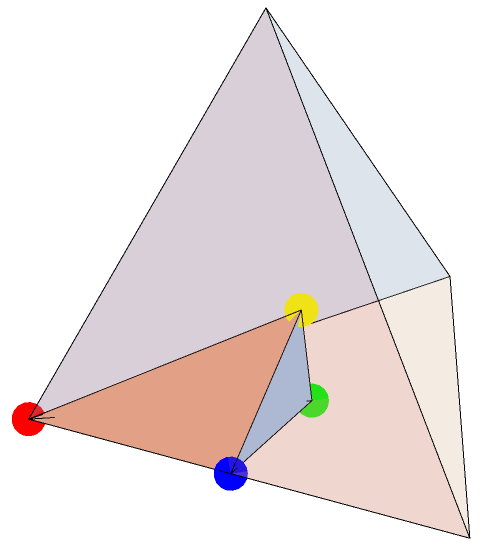
\includegraphics[width=0.6\linewidth]{p5}
	\end{subfigure}
	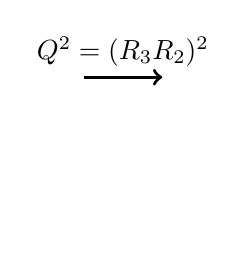
\begin{tikzpicture}
		\draw[->,very thick] (0,0)--(1,0) node[midway, above] {$Q^2=(R_3R_2)^2$};;
		\filldraw[white] (0,-2) circle (0.05);
	\end{tikzpicture}
	\begin{subfigure}{0.5\linewidth}
		\centering
		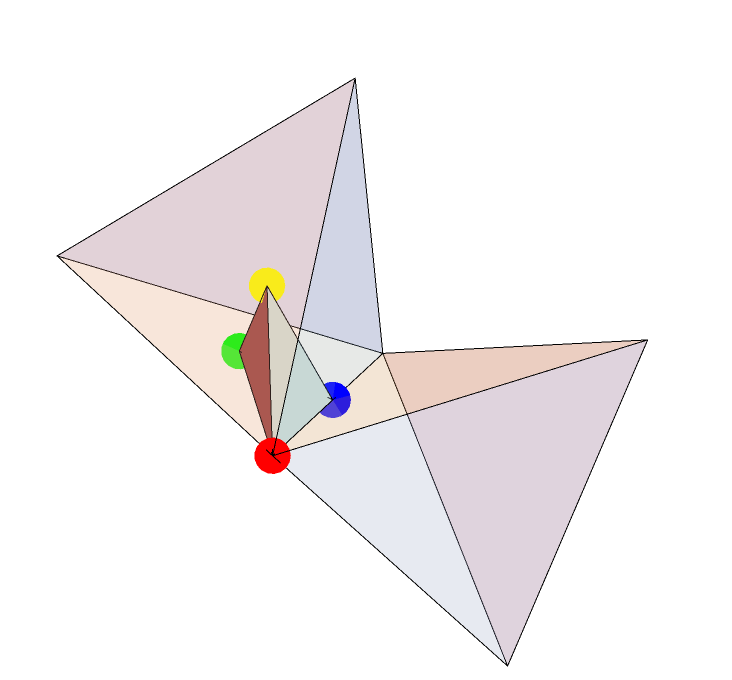
\includegraphics[width=0.9\linewidth]{p6}
	\end{subfigure}
	\end{figure}
	Ahora rotemos respecto a la recta amarillo-verde en dirección horaria (vista desde arriba), $R_0R_1$:
	\begin{figure}[H]
	\begin{subfigure}{0.4\linewidth}
		\centering
		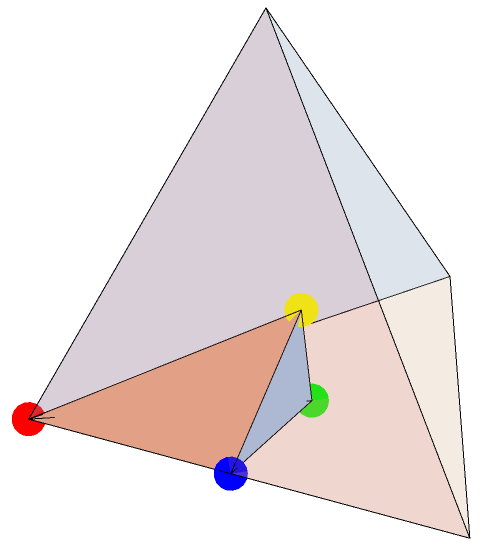
\includegraphics[width=0.6\linewidth]{p5}
	\end{subfigure}
	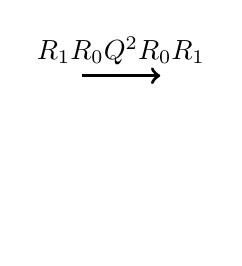
\begin{tikzpicture}
		\draw[->,very thick] (0,0)--(1,0) node[midway, above] {$R_1R_0Q^2R_0R_1$};;
		\filldraw[white] (0,-2) circle (0.05);
	\end{tikzpicture}
	\begin{subfigure}{0.4\linewidth}
		\centering
		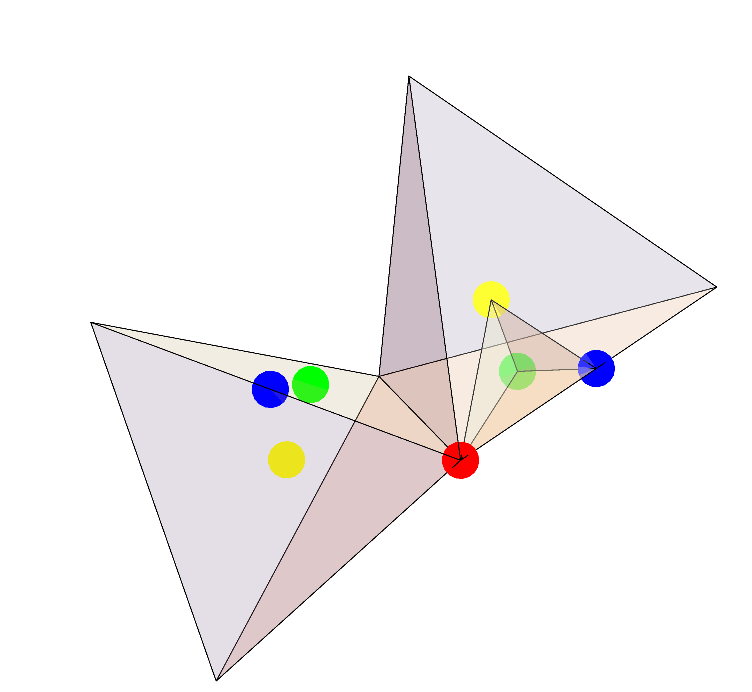
\includegraphics[width=0.9\linewidth]{p7}
	\end{subfigure}
\end{figure}
	Hemos destacado a dónde van a dar los puntos azul, amarillo y verde, que corresponden al plano de reflexión de $R_0$. Definamos 
	\begin{align*}
		P_1&=(R_1R_0Q^2R_0R_1)^{-1}R_0(R_1R_0Q^2R_0R_1)\\
		&=(R_1R_0(R_3R_2)^2R_0R_1)^{-1}R_0(R_1R_0(R_3R_2)^2R_0R_1)\\
		&=(R_1R_0R_3R_2R_3R_2R_0R_1)^{-1}R_0(R_1R_0R_3R_2R_3R_2R_0R_1)\\
		&=R_1R_0R_2R_3R_2R_3R_0R_1R_0R_1R_0R_3R_2R_3R_2R_0R_1\\
		&=R_1R_0R_2R_3R_2R_3R_1R_0R_1R_1R_0R_3R_2R_3R_2R_0R_1\\	&=R_1R_0R_2R_3R_2R_3R_1R_3R_2R_3R_2R_0R_1\\
		&=R_1R_0R_2R_3R_2R_1R_3R_3R_2R_3R_2R_0R_1\\
		&=R_1R_0R_2R_3R_2R_1R_2R_3R_2R_0R_1
	\end{align*}
	
%	La rotación por la arista rojo-amarillo es $R_2R_1$. Al conjugarla por la rotación del centro de la cara (clockwise desde arriba, es $R_0R_2$), obtenemos $Q=(R_0R_2)^{-1}R_2R_1(R_0R_2)$, que es la rotación por la línea por el centro de la cara (amarillo) y el vértice que está en frente del azul. Conjugamos $R_3$ por esta rotación para obtener la reflexión por la cara izquierda del tetraedro, $Q_2=Q^{-1}R_3Q$. Y finalmente conjugamos $R_0$ por $Q_2$.
%	\begin{align*}
%		P_1&=Q_2R_0Q_2\\
%		&=Q^{-1}R_3QR_0Q^{-1}R_3Q\\
%		&=R_2R_0R_1R_2R_0R_1R_3R_2R_0R_2R_1R_0R_2R_0R_2R_0R_1R_2R_0R_1R_3R_2R_0R_2R_1R_0R_2
%	\end{align*}
%	ya que $Q^{-1}=R_2R_0R_1R_2R_0R_1$.
%
%\begin{align*}
%	R_2R_3R_2R_3R_2R_3R_2R_3R_2R_3&=1\\
%	R_3R_2R_3R_2R_3R_2R_3&=R_2R_3R_2
%\end{align*}

	Ahora veamos que se satisfacen las relaciones. Sustituyendo,
	\[(P_0P_2)^2=(R_0R_3)^2=1\qquad (P_0P_3)^2=(R_0R_2)^2=1\qquad (P_2P_3)^5=(R_3R_2)^5=1\]

\end{proof}

Ahora
\begin{itemize}
	\item Sustituir en las fórmulas de las $S_i$ pero usando estas $P_i$.
	\item Ya sabemos que cuando haces esto queda un poliedro.
	\item Hay que buscar una $S_3$. ¿Qué necesitas que cumpla? Bueno, $S_1S_2$ es el medio giro en la arista o en la arista adyacente(depende del orden)
	\item Necesitas:
	\begin{itemize}
		\item $(S_1S_2S_3)^2=1$ [Pensamos que esta es giro de brocheta por un palillo que va del vértice al centro de la cara]
		\item $(S_2S_3)^2=1$.
			\item Y después $vS_3=v$
		\item $eS_3=v$
	\end{itemize}
\end{itemize}

\section{En busca de otros poliedros quirales}
Esta sección es una transcripción del trabajo de Bris.

\subsection{Definiciones y resultados}
Damos algunas definiciones, explicamos el método básico para construir poliedros usando la construcción de Wythoff y mostramos un par de teoremas.

\begin{defn}
	Un \textbf{polígono (geométrico)} en $\R^d$ es:
	\begin{itemize}
		\item Un conjunto discreto de puntos llamados \textbf{vértices}
		\item Un conjunto de segmentos que los unen llamados \textbf{aristas}
	\end{itemize}
	tales que la gráfica resultante es 2-regular.
\end{defn}

\begin{defn}
	Un \textbf{poliedro (geométrico)} en $R^d$ es un conjunto de polígonos llamados \textbf{caras} tal que:
	\begin{itemize}
		\item Los vértices son un conjunto discreto
		\item Cada arista pertenece exactamente a dos caras.
		\item La gráfica determinada por los vértices y las aristas es conexa.
		\item La figura de vértice en cada vértice es un polígono.
	\end{itemize}
\end{defn}

\begin{defn}[Banderas]
	\begin{itemize}
		\item 	Una \textbf{bandera} de un poliedro es un vértice, una arista y una cara mutualmente incidentes.
		\item Si $\Phi$ es una bandera, $\mathbf{\Phi^i}$ es la bandera que difiere de $\Phi$ sólo por en la cara $i\in\{0,1,2\}$ y se llama la $i$\textbf{-bandera adyacente}.
	\end{itemize}
\end{defn}

\begin{defn}
	Un poliedro $\mathcal{P}$ es \textbf{(geométricamente) quiral} si $G(\mathcal{P}$ induce dos órbitas en banderas y las banderas adyacentes están en órbitas distintas.
\end{defn}
\begin{obs}
	Un poliedro geométricamente quiral puede ser combinatoriamente quiral o regular.
\end{obs}

\begin{Wreg}Sean $R_0,R_1$ y $R_2$ isometrías en $\R^n$ que queremos usar para construir un poliedro regular $\p$  y sea $G=\langle R_0,R_1,R_2\rangle$. Ahora
\begin{itemize}
	\item Escogemos un vértice $v$ que será el \textbf{vértice base} de $\p$ tal que $v\in\Fix R_1\cap\Fix R_2$ y $v\notin\Fix R_0$.
	\item La \textbf{arista base} es el segmento de línea que une $v$ con $vR_0$.
	\item La \textbf{cara base} es la órbita de $v$ y $e$ bajo $\langle R_1,R_1\rangle$.
\end{itemize}
Luego,
\begin{align*}
	V&:=\{vR:R\in G\}\text{ son los vértices de } \p.\\ 
	E&:=\{eR:R\in G\} \text{ son las aristas de } \p.\\ 
	F&:=\{fR:R\in G\} \text{ son las caras de } \p.
\end{align*}
Esta estructura se nota por $\p$ o $\p(R_0,R_1,R_2;v)$
\end{Wreg}

\begin{Wqui}
	Sean $S_1$ y $S_2$ isometrías en $\R^n$ que queremos usar para construir un poliedro quiral $\p$  y sea $G=\langle S_1,S_2\rangle$. Ahora
	\begin{itemize}
		\item Necesitamos suponer que $(S_1S_2)^2=1$.
		\item Escogemos un vértice $v$ que será el \textbf{vértice base} de $\p$ tal que $v\in\Fix S_2$ y $v\notin\Fix S_1$.
		\item La \textbf{arista base} es el segmento de línea que une $v$ con $vS_1^{-1}=vS_2^{-1}S_1^{-1}=vS_1S_2$. Necesitamos suponer que $eS_1\neq e$ y $eS_2\neq e$.
		\item La \textbf{cara base} es $\{vS,eS:S\in\langle S_1\rangle\}$. Necesitamos suponer que $fS_2\neq f$.
	\end{itemize}
	Luego,
	\begin{align*}
		V&:=\{vR:R\in G\}\text{ son los vértices de } \p.\\ 
		E&:=\{eR:R\in G\} \text{ son las aristas de } \p.\\ 
		F&:=\{fR:R\in G\} \text{ son las caras de } \p.
	\end{align*}
	Esta estructura se nota por $\p$ o $\p(S_1,S_2;v)$.
\end{Wqui}

\paragraph{¿Cómo podemos estar seguros de que esta construcción nos da un poliedro?}
\begin{teo}\label{teo:bris1}
	Sea $G=\langle S_1,S_2\rangle$ un grupo discreto, donde $S_1$ y $S_2$ son isometrías de $\R^n$ tales que $(S_1S_2)^2=1$ y sea $\p=\p(S_1,S_2;v)$. Supongamos que se satisfacen las siguientes condiciones:
	\begin{itemize}
		\item $\langle S_1\rangle\cap\langle S_2\rangle=\{1\}$.
		\item $S_1$ y $S_2$ son de orden mayor estricto que 2.
		\item $\Stab_G v=\langle S_2\rangle$, $\Stab_G e=\langle S_1S_2\rangle$ y $\Stab_G f=\langle S_1\rangle$.
	\end{itemize}
	Entones $\p$ es un poliedro geométrico regular o quiral cuyo grupo de simetrías ``es $G$ como un subgrupo de índice 2 en $G(\p)$".
\end{teo}

\begin{teo}[Bracho, Hubard, Pellicer]
	$\p$ es un poliedro quiral en $\s^3$ si y sólo si se satisface alguna de las siguientes condiciones:
	\begin{itemize}
		\item $\p$ tiene caras holanes y figuras de vértices holanes.
		\item $\p$ tiene caras helicoidales y figuras de vértice planas, y el plano que contiene a la figura de vértice de $v$ no contiene a $v$.
	\end{itemize}
\end{teo}
\begin{obs}
	En el segundo caso, si el vértice está en la figura de vértice, el poliedro es regular.
\end{obs}

\subsection{Looking for chiral polyhedra}
El trabajo de Bris está planteado de la siguiente manera:

Sean $\T=\{p,q,r\}$ un 4-politopo regular esférico y $R_0,R_1,R_2$ y $R_3$ las isometrías que generan a $\T$ con respecto a $\Phi$. Denotaremos $[p,q,r]:=\langle R_0,R_1,R_2,R_3\rangle$.

Escogemos un vértice $v$ y una arista $e$ de $\T$ para construir un poliedro usando el método de Wythoff, es decir, queremos que $v$ y $e$ estén en $\p(S_1,S_2;v)$.

Definimos $S_1=R_0R_1R_2R_3$ (recordemos que $\Stab f=\langle S_1\rangle$ en el teorema).  La arista $e$ es el segmento de línea que une $v$ con $vS_1^{-1}$. Luego, la cara $f=\{v,e\}\langle S_1\rangle$ es un \textbf{polígono de petrie}.

El objetivo es encontrar una $S_2$ con figuras de vértice planas, y tales que contienen al vértice del cual son la figura de vértice. Como queremos usar el teorema, tendremos que $v\in\Fix S_2$, así que debemos buscar $S_2$ en $\langle R_1,R_2,R_3\rangle$.

Se obtuvieron los siguientes resultados:

\begin{center}
	\begin{tabular}{|c |c| c| c|c|}
	\hline
	\multicolumn{5}{|c|}{\textbf{Poliedros quirales con caras Petrie}}\\
	\hline\textbf{4-politopo $\T$} & \textbf{Poliedro} $\p$ &$S_1$&$S_2$&$|\langle S_1,S_2\rangle|$\\\hline\hline
	$\{3,3,3\}$&—&\multirow{8}{*}{$R_0R_1R_2R_3$}&—&—\\		\cline{1-2}\cline{4-5}
	$\{3,3,4\}$&$\{8,4\}$&&$R_3R_2R_1R_2$&32\\\cline{1-2}	\cline{4-5}
	\multirow{2}{*}{$\{4,3,3\}$}&\multirow{2}{*}{$\{8,3\}$}&&$R_3R_2R_1R_3$&\multirow{2}{*}{48}\\
	&&&$R_3R_2R_1R_2$&\\\cline{1-2}	\cline{4-5}
	$\{3,4,3\}$&—&&—&—\\\cline{1-2}	\cline{4-5}
	$\{3,3,5\}$&—&&—&—\\\cline{1-2}	\cline{4-5}
	\multirow{2}{*}{$\{5,3,3\}$}&\multirow{2}{*}{$\{30,3\}$}&&$R_3R_2R_1R_3$&\multirow{2}{*}{1440}\\
	&&&$R_3R_2R_1R_2$&\\\hline
\end{tabular}
\end{center}

Después de esto hubo una búsqueda por poliedros quirales con caras helicoidales:

\begin{center}
	\begin{tabular}{|c |c| c| c|c|}
		\hline
		\multicolumn{5}{|c|}{\textbf{Poliedros quirales con caras helicoidales}}\\
		\hline\textbf{4-politopo $\T$} & \textbf{Poliedro} $\p$ &$S_1$&$S_2$&$|\langle S_1,S_2\rangle|$\\\hline\hline
		$\{3,3,3\}$&—&—&—&—\\\hline
		$\{3,3,4\}$&—&—&—&—\\\hline
		\multirow{2}{*}{$\{3,3,5\}$}&\multirow{2}{*}{$\{12,3\}$}&\multirow{2}{*}{$(R_1R_2R_3)^3R_0$}&$R_2R_3(R_2R_3R_1)^2R_2R_1$&\multirow{2}{*}{144}\\
		&&&$R_3R_2R_3R_1R_2R_3R_2R_1$&\\
		\hline
	\end{tabular}
\end{center}
\end{document}

%DIBUJO DEL CUBO DE ROLI
%\begin{tikzpicture}[scale=1.3, tdplot_main_coords, line width=2pt, line cap=round]
%	% Define cube coordinates for the inner cube (smaller size)
%	\coordinate[label=above right:$A$] (A) at (-0.5,-0.5,-0.5);
%	\coordinate[label=above right:$B$] (B) at (-0.5,0.5,-0.5);
%	\coordinate[label=above left:$C$] (C) at (0.5,0.5,-0.5);
%	\coordinate[label=above left:$D$] (D) at (0.5,-0.5,-0.5);
%	\coordinate[label=below right:$E$] (E) at (-0.5,-0.5,0.5);
%	\coordinate[label=below right:$F$] (F) at (-0.5,0.5,0.5);
%	\coordinate[label=below left:$G$] (G) at (0.5,0.5,0.5);
%	\coordinate[label=below left:$H$] (H) at (0.5,-0.5,0.5);
%	
%	% Define cube coordinates for the outer cube (larger size)
%	\coordinate[label=above right:$A'$] (A2) at (-1.5,-1.5,-1.5);
%	\coordinate[label=above right:$B'$] (B2) at (-1.5,1.5,-1.5);
%	\coordinate[label=above left:$C'$] (C2) at (1.5,1.5,-1.5);
%	\coordinate[label=above left:$D'$] (D2) at (1.5,-1.5,-1.5);
%	\coordinate[label=below right:$E'$] (E2) at (-1.5,-1.5,1.5);
%	\coordinate[label=below right:$F'$] (F2) at (-1.5,1.5,1.5);
%	\coordinate[label=below left:$G'$] (G2) at (1.5,1.5,1.5);
%	\coordinate[label=below left:$H'$] (H2) at (1.5,-1.5,1.5);
%	
%	% Draw lines connecting the inner and outer cube vertices
%	\draw[limegreen] (A) -- (A2);
%	\draw[limegreen] (B) -- (B2);
%	\draw[limegreen] (C) -- (C2);
%	\draw[limegreen] (D) -- (D2);
%	\draw[limegreen] (E) -- (E2);
%	\draw[limegreen] (F) -- (F2);
%	\draw[limegreen] (G) -- (G2);
%	\draw[limegreen] (H) -- (H2);
%	
%	% Draw inner cube edges (smaller size) with random colors
%	%Z
%	\draw[blue-violet] (A) -- (E);
%	\draw[blue-violet] (B) -- (F);
%	\draw[blue-violet] (C) -- (G);
%	\draw[blue-violet] (D) -- (H);
%	%X
%	\draw[blue] (B) -- (C);
%	\draw[blue] (D) -- (A);
%	\draw[blue] (F) -- (G);
%	\draw[blue] (H) -- (E);
%	%Y
%	\draw[red] (C) -- (D);
%	\draw[red] (A) -- (B);
%	\draw[red] (E) -- (F);
%	\draw[red] (G) -- (H);
%	
%	% Draw outer cube edges with random colors
%	%Z
%	\draw[blue-violet] (A2) -- (E2);
%	\draw[blue-violet] (B2) -- (F2);
%	\draw[blue-violet] (C2) -- (G2);
%	\draw[blue-violet] (D2) -- (H2);
%	%X
%	\draw[blue] (B2) -- (C2);
%	\draw[blue] (D2) -- (A2);
%	\draw[blue] (F2) -- (G2);
%	\draw[blue] (H2) -- (E2);
%	%Y
%	\draw[red] (C2) -- (D2);
%	\draw[red] (A2) -- (B2);
%	\draw[red] (E2) -- (F2);
%	\draw[red] (G2) -- (H2);
%\end{tikzpicture}